\documentclass[11pt]{article}
\usepackage[utf8]{inputenc}
\usepackage{geometry}
\usepackage{array}
\usepackage{booktabs}
\usepackage{longtable}
\usepackage{xcolor}
\usepackage{colortbl}
\usepackage{fancyhdr}
\usepackage{titlesec}
\usepackage{tcolorbox}
\usepackage{enumitem}
\usepackage{graphicx}

\geometry{margin=0.75in, top=1in, bottom=1in}

% Define custom colors
\definecolor{primaryblue}{RGB}{41, 128, 185}
\definecolor{accentorange}{RGB}{230, 126, 34}
\definecolor{darkgray}{RGB}{52, 73, 94}
\definecolor{lightgray}{RGB}{236, 240, 241}
\definecolor{tableheader}{RGB}{52, 152, 219}
\definecolor{tableodd}{RGB}{250, 250, 250}

% Configure section titles
\titleformat{\section}
  {\normalfont\LARGE\bfseries\color{primaryblue}}
  {\thesection}{1em}{}[\titlerule]
  
\titleformat{\subsection}
  {\normalfont\Large\bfseries\color{darkgray}}
  {\thesubsection}{1em}{}
  
\titleformat{\subsubsection}
  {\normalfont\large\bfseries\color{accentorange}}
  {\thesubsubsection}{1em}{}

% Configure header and footer
\pagestyle{fancy}
\fancyhf{}
\fancyhead[L]{\small\color{darkgray}GIU Food Truck Management System}
\fancyhead[R]{\small\color{darkgray}Database Tables Specification}
\fancyfoot[C]{\small\color{darkgray}\thepage}
\renewcommand{\headrulewidth}{0.5pt}
\renewcommand{\footrulewidth}{0.5pt}

% Configure lists
\setlist[itemize]{leftmargin=*, itemsep=3pt, parsep=0pt}
\setlist[enumerate]{leftmargin=*, itemsep=3pt, parsep=0pt}

\title{\vspace{-1cm}\Huge\textbf{\color{primaryblue}GIU Food Truck Management System}\\\vspace{0.3cm}\LARGE\color{darkgray}Database Tables Specification}
\author{}
\date{\vspace{-0.5cm}}

\begin{document}

% ============================================
% COVER PAGE
% ============================================
\begin{titlepage}
    \centering
    \vspace*{2cm}
    
    % Top decorative line
    {\color{primaryblue}\rule{\textwidth}{2pt}}
    
    \vspace{1.5cm}
    
    % Main Title
    {\Huge\bfseries\color{primaryblue} Database Tables\\[0.3cm] Specification}
    
    \vspace{0.8cm}
    
    % Subtitle
    {\LARGE\color{darkgray} GIU Food Truck\\[0.2cm] Management System}
    
    \vspace{1cm}
    
    {\color{accentorange}\rule{0.6\textwidth}{1.5pt}}
    
    \vspace{2cm}
    
    % Team Information Box
    \begin{tcolorbox}[colback=lightgray, colframe=primaryblue, boxrule=1.5pt, arc=4mm, width=0.8\textwidth]
        \centering
        {\Large\bfseries\color{darkgray} Team Sleepers}
        
        \vspace{0.8cm}
        
        \begin{tabular}{p{6cm}p{3cm}}
            Hassan Yousef & 13006567 \\ 
            Sara Adel & 14003723 \\
            Hana Yasser & 13003628 \\
            Mohamed Walid & 13006513 \\
            Omar Hani & 13007515 \\
            Abdelhamid ElSharnouby & 13006294 \\
            Hanin Mohamed & 13007010 \\
            Khaled Khaled & 14001048 \\
        \end{tabular}
    \end{tcolorbox}
    
    \vspace{2cm}
    
    % University Information
    \begin{tcolorbox}[colback=white, colframe=accentorange, boxrule=1pt, arc=3mm, width=0.7\textwidth]
        \centering
        {\large\bfseries German International University (GIU)}
        
        \vspace{0.5cm}
        
        {\normalsize\textbf{Supervised by:}}\\[0.3cm]
        Dr.~Iman Awaad\\
        Eng.~Amir Haytham
    \end{tcolorbox}
    
    \vfill
    
    % Date and Version
    \begin{tcolorbox}[colback=primaryblue!10, colframe=primaryblue, boxrule=0.8pt, arc=2mm, width=0.5\textwidth]
        \centering
        {\large\bfseries\color{darkgray}\today}\\[0.2cm]
        {\small Version 1.0}
    \end{tcolorbox}
    
    \vspace{1cm}
    
    % Bottom decorative line
    {\color{primaryblue}\rule{\textwidth}{2pt}}
    
\end{titlepage}

% ============================================
% DOCUMENT OVERVIEW
% ============================================
\thispagestyle{fancy}

\begin{tcolorbox}[colback=lightgray, colframe=primaryblue, boxrule=1pt, arc=3mm]
\textbf{\large Overview:} This document provides a comprehensive list of all database tables in the GIU Food Truck Management System, including their columns, primary keys, foreign keys, and relationship attributes.
\end{tcolorbox}

\vspace{0.5cm}

\section{Entity-Relationship Diagram}

\begin{figure}[h]
\centering
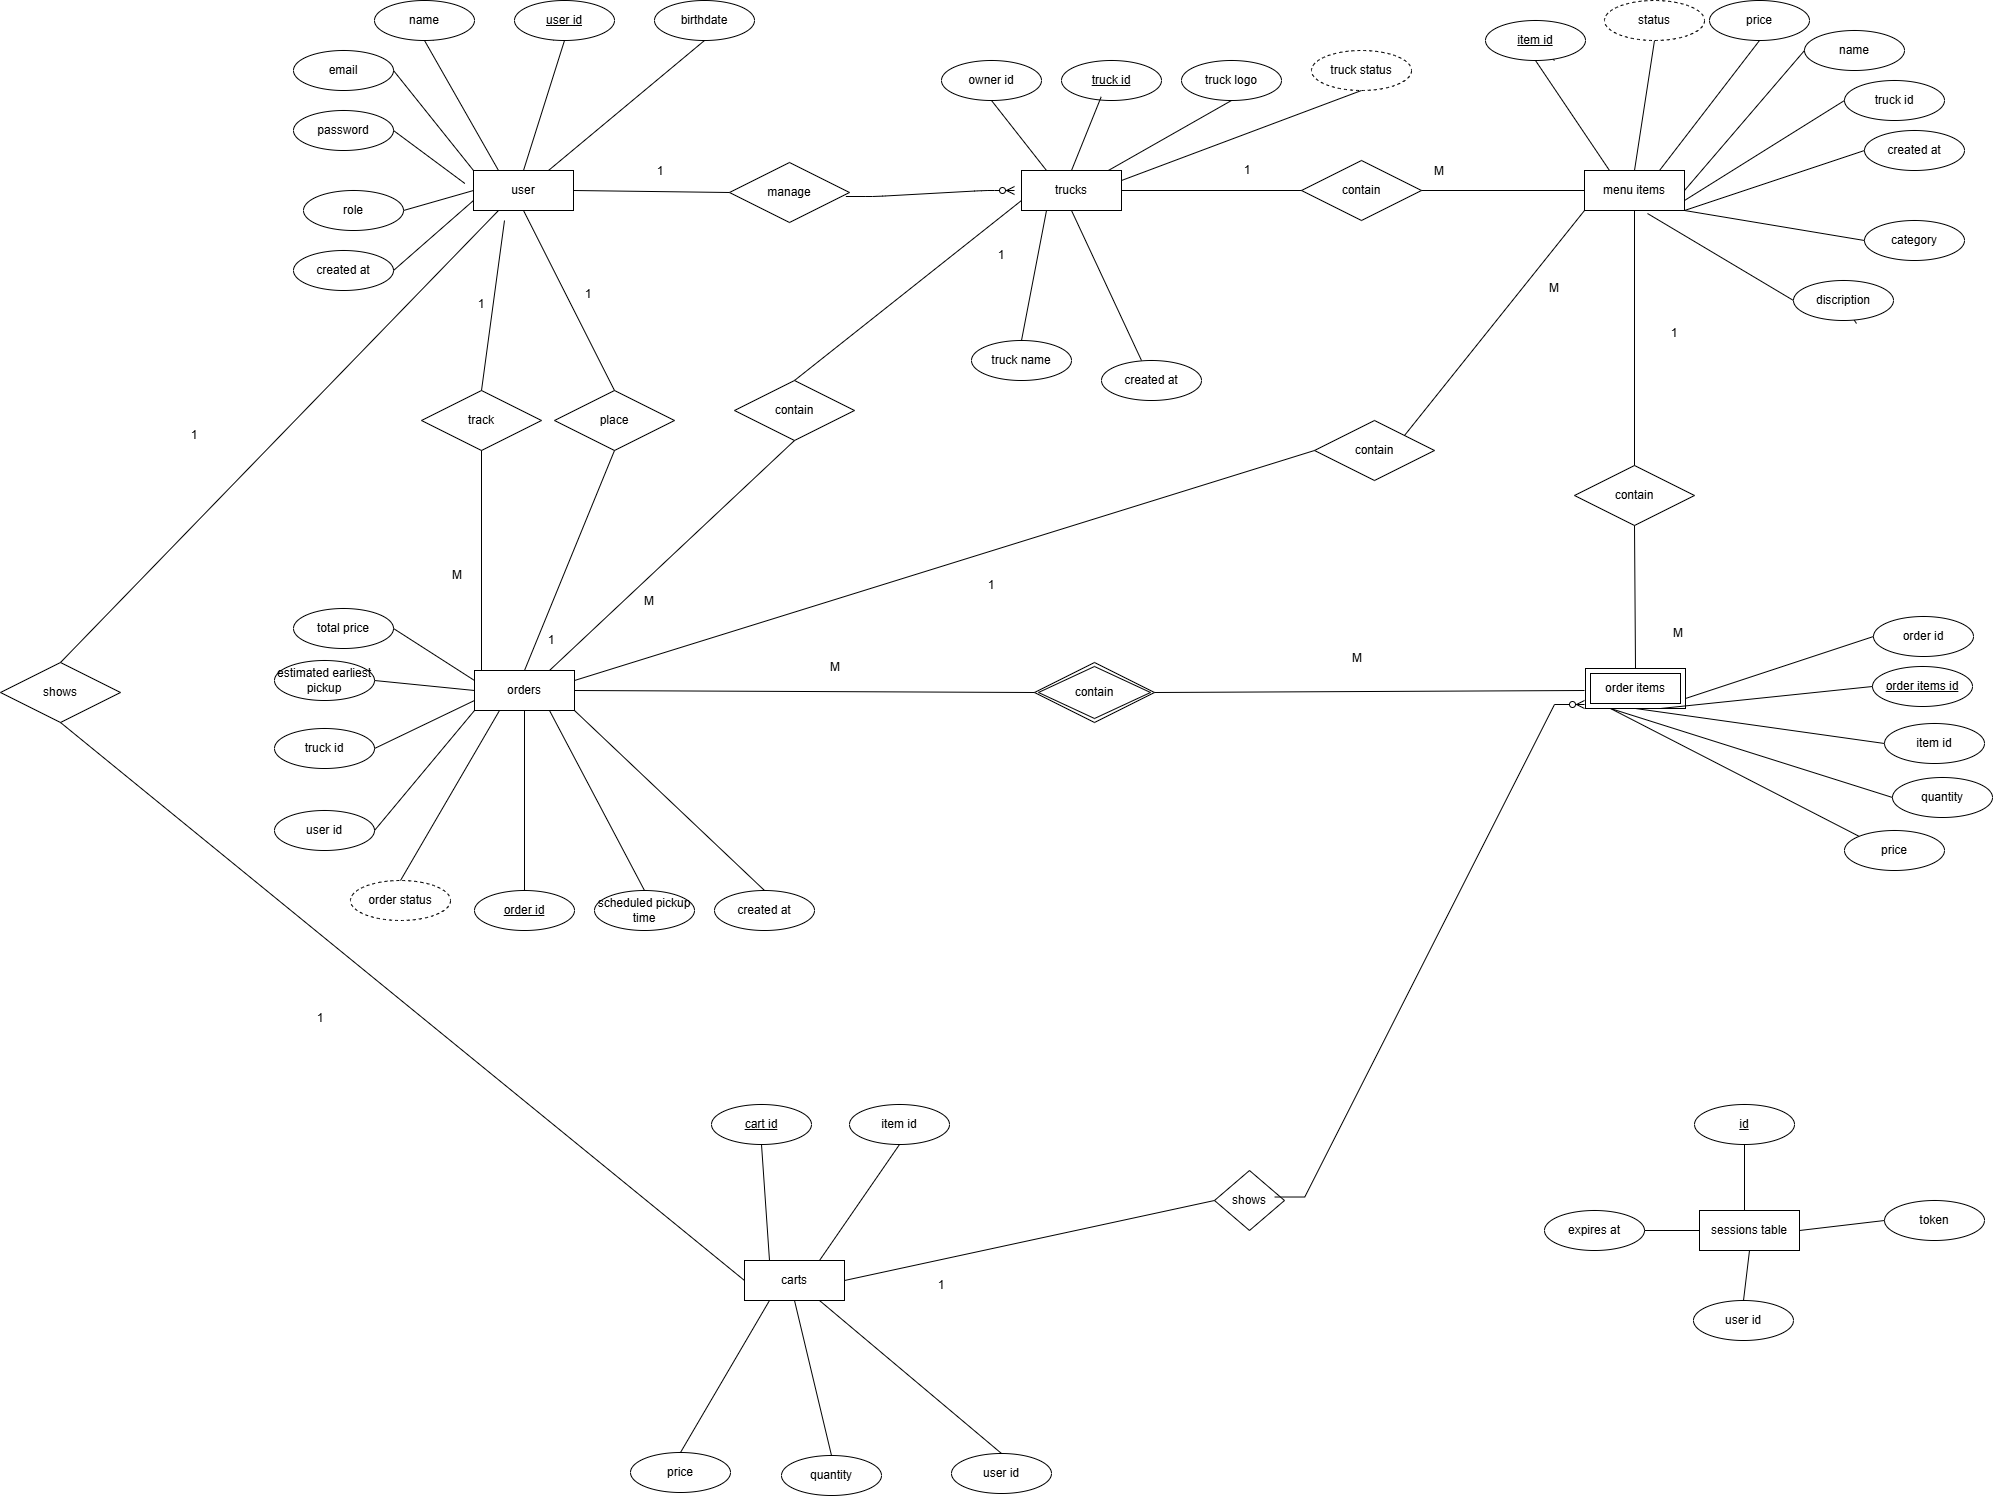
\includegraphics[width=\textwidth,keepaspectratio]{ERD Diagram.drawio (1).png}
\caption{GIU Food Truck Management System - Entity-Relationship Diagram}
\label{fig:erd}
\end{figure}

\vspace{0.5cm}

\section{Database Tables Overview}

This document describes the complete database schema with \textbf{7 Entity Tables} and \textbf{8 Junction Tables} (15 tables total).

\subsection{Entity Tables}

The following 7 tables represent the core entities in the system:

\subsubsection{1. Users Table}

\begin{tcolorbox}[colback=white, colframe=accentorange, boxrule=0.5pt, arc=2mm, left=3mm, right=3mm]
\textbf{Table Name:} \texttt{FoodTruck.Users}\\
\textbf{Description:} Stores information about system users (customers and truck owners).
\end{tcolorbox}

\vspace{0.3cm}

\begin{longtable}{|>{\columncolor{white}}p{3cm}|>{\columncolor{white}}p{2.3cm}|>{\columncolor{white}}p{7.5cm}|}
\hline
\rowcolor{tableheader}
\textcolor{white}{\textbf{Column Name}} & \textcolor{white}{\textbf{Data Type}} & \textcolor{white}{\textbf{Description}} \\
\hline
\endfirsthead
\hline
\rowcolor{tableheader}
\textcolor{white}{\textbf{Column Name}} & \textcolor{white}{\textbf{Data Type}} & \textcolor{white}{\textbf{Description}} \\
\hline
\endhead
\rowcolor{tableodd}
userId & serial & \textbf{\color{primaryblue}Primary Key} - Unique identifier for each user \\
\hline
name & text & User's full name (NOT NULL) \\
\hline
\rowcolor{tableodd}
email & text & User's email address (NOT NULL, UNIQUE) \\
\hline
password & text & Hashed password (NOT NULL) \\
\hline
\rowcolor{tableodd}
role & text & User role: 'customer' or 'truckOwner' (DEFAULT: 'customer') \\
\hline
birthDate & date & User's date of birth (DEFAULT: current\_timestamp) \\
\hline
\rowcolor{tableodd}
createdAt & timestamp & Account creation timestamp (DEFAULT: current\_timestamp) \\
\hline
\end{longtable}

\vspace{0.5cm}

\subsubsection{2. Trucks Table}

\begin{tcolorbox}[colback=white, colframe=accentorange, boxrule=0.5pt, arc=2mm, left=3mm, right=3mm]
\textbf{Table Name:} \texttt{FoodTruck.Trucks}\\
\textbf{Description:} Stores information about food trucks.
\end{tcolorbox}

\vspace{0.3cm}

\begin{longtable}{|>{\columncolor{white}}p{3cm}|>{\columncolor{white}}p{2.3cm}|>{\columncolor{white}}p{7.5cm}|}
\hline
\rowcolor{tableheader}
\textcolor{white}{\textbf{Column Name}} & \textcolor{white}{\textbf{Data Type}} & \textcolor{white}{\textbf{Description}} \\
\hline
\endfirsthead
\hline
\rowcolor{tableheader}
\textcolor{white}{\textbf{Column Name}} & \textcolor{white}{\textbf{Data Type}} & \textcolor{white}{\textbf{Description}} \\
\hline
\endhead
\rowcolor{tableodd}
truckId & serial & \textbf{\color{primaryblue}Primary Key} - Unique identifier for each truck \\
\hline
truckName & text & Name of the food truck (NOT NULL, UNIQUE) \\
\hline
\rowcolor{tableodd}
truckLogo & text & URL to truck logo image \\
\hline
ownerId & integer & \textbf{\color{accentorange}Foreign Key} references Users(userId) - Owner of the truck (NOT NULL) \\
\hline
\rowcolor{tableodd}
truckStatus & text & Operating status: 'available', 'unavailable' (DEFAULT: 'available') \\
\hline
orderStatus & text & Order acceptance status: 'available', 'unavailable' (DEFAULT: 'available') \\
\hline
\rowcolor{tableodd}
createdAt & timestamp & Truck registration timestamp (DEFAULT: current\_timestamp) \\
\hline
\end{longtable}

\begin{tcolorbox}[colback=lightgray, colframe=darkgray, boxrule=0.5pt, arc=2mm, left=3mm]
\textbf{Foreign Key Constraints:}
\begin{itemize}[leftmargin=1cm]
    \item ownerId REFERENCES Users(userId) ON DELETE CASCADE
\end{itemize}
\end{tcolorbox}

\vspace{0.5cm}

\subsubsection{3. MenuItems Table}

\begin{tcolorbox}[colback=white, colframe=accentorange, boxrule=0.5pt, arc=2mm, left=3mm, right=3mm]
\textbf{Table Name:} \texttt{FoodTruck.MenuItems}\\
\textbf{Description:} Stores menu items for each food truck.
\end{tcolorbox}

\vspace{0.3cm}

\begin{longtable}{|>{\columncolor{white}}p{3cm}|>{\columncolor{white}}p{2.3cm}|>{\columncolor{white}}p{7.5cm}|}
\hline
\rowcolor{tableheader}
\textcolor{white}{\textbf{Column Name}} & \textcolor{white}{\textbf{Data Type}} & \textcolor{white}{\textbf{Description}} \\
\hline
\endfirsthead
\hline
\rowcolor{tableheader}
\textcolor{white}{\textbf{Column Name}} & \textcolor{white}{\textbf{Data Type}} & \textcolor{white}{\textbf{Description}} \\
\hline
\endhead
\rowcolor{tableodd}
itemId & serial & \textbf{\color{primaryblue}Primary Key} - Unique identifier for each menu item \\
\hline
truckId & integer & \textbf{\color{accentorange}Foreign Key} references Trucks(truckId) - Associated truck (NOT NULL) \\
\hline
\rowcolor{tableodd}
name & text & Name of the menu item (NOT NULL) \\
\hline
description & text & Detailed description of the item \\
\hline
\rowcolor{tableodd}
price & numeric(10,2) & Price of the item (NOT NULL) \\
\hline
category & text & Category: 'Main Course', 'Sides', 'Beverages', etc. (NOT NULL) \\
\hline
\rowcolor{tableodd}
status & text & Availability status: 'available', 'unavailable' (DEFAULT: 'available') \\
\hline
createdAt & timestamp & Item creation timestamp (DEFAULT: current\_timestamp) \\
\hline
\end{longtable}

\begin{tcolorbox}[colback=lightgray, colframe=darkgray, boxrule=0.5pt, arc=2mm, left=3mm]
\textbf{Foreign Key Constraints:}
\begin{itemize}[leftmargin=1cm]
    \item truckId REFERENCES Trucks(truckId) ON DELETE CASCADE
\end{itemize}
\end{tcolorbox}

\vspace{0.5cm}

\subsubsection{4. Orders Table}

\begin{tcolorbox}[colback=white, colframe=accentorange, boxrule=0.5pt, arc=2mm, left=3mm, right=3mm]
\textbf{Table Name:} \texttt{FoodTruck.Orders}\\
\textbf{Description:} Stores customer orders.
\end{tcolorbox}

\vspace{0.3cm}

\begin{longtable}{|>{\columncolor{white}}p{3cm}|>{\columncolor{white}}p{2.3cm}|>{\columncolor{white}}p{7.5cm}|}
\hline
\rowcolor{tableheader}
\textcolor{white}{\textbf{Column Name}} & \textcolor{white}{\textbf{Data Type}} & \textcolor{white}{\textbf{Description}} \\
\hline
\endfirsthead
\hline
\rowcolor{tableheader}
\textcolor{white}{\textbf{Column Name}} & \textcolor{white}{\textbf{Data Type}} & \textcolor{white}{\textbf{Description}} \\
\hline
\endhead
\rowcolor{tableodd}
orderId & serial & \textbf{\color{primaryblue}Primary Key} - Unique identifier for each order \\
\hline
userId & integer & \textbf{\color{accentorange}Foreign Key} references Users(userId) - Customer who placed the order (NOT NULL) \\
\hline
\rowcolor{tableodd}
truckId & integer & \textbf{\color{accentorange}Foreign Key} references Trucks(truckId) - Truck fulfilling the order (NOT NULL) \\
\hline
orderStatus & text & Order status: 'pending', 'confirmed', 'ready', 'completed', 'cancelled' (NOT NULL) \\
\hline
\rowcolor{tableodd}
totalPrice & numeric(10,2) & Total price of the order (NOT NULL) \\
\hline
scheduled\-Pickup\-Time & timestamp & Customer's preferred pickup time \\
\hline
\rowcolor{tableodd}
estimated\-Earliest\-Pickup & timestamp & Estimated earliest pickup time \\
\hline
createdAt & timestamp & Order creation timestamp (DEFAULT: current\_timestamp) \\
\hline
\end{longtable}

\begin{tcolorbox}[colback=lightgray, colframe=darkgray, boxrule=0.5pt, arc=2mm, left=3mm]
\textbf{Foreign Key Constraints:}
\begin{itemize}[leftmargin=1cm]
    \item userId REFERENCES Users(userId) ON DELETE CASCADE
    \item truckId REFERENCES Trucks(truckId) ON DELETE CASCADE
\end{itemize}
\end{tcolorbox}

\vspace{0.5cm}

\subsubsection{5. OrderItems Table}

\begin{tcolorbox}[colback=white, colframe=accentorange, boxrule=0.5pt, arc=2mm, left=3mm, right=3mm]
\textbf{Table Name:} \texttt{FoodTruck.OrderItems}\\
\textbf{Description:} Stores individual line items within an order. Each record represents one menu item with its quantity and price in an order.
\end{tcolorbox}

\vspace{0.3cm}

\begin{longtable}{|>{\columncolor{white}}p{3cm}|>{\columncolor{white}}p{2.3cm}|>{\columncolor{white}}p{7.5cm}|}
\hline
\rowcolor{tableheader}
\textcolor{white}{\textbf{Column Name}} & \textcolor{white}{\textbf{Data Type}} & \textcolor{white}{\textbf{Description}} \\
\hline
\endfirsthead
\hline
\rowcolor{tableheader}
\textcolor{white}{\textbf{Column Name}} & \textcolor{white}{\textbf{Data Type}} & \textcolor{white}{\textbf{Description}} \\
\hline
\endhead
\rowcolor{tableodd}
orderItemId & serial & \textbf{\color{primaryblue}Primary Key} - Unique identifier for each order item \\
\hline
name & text & Name/description of the ordered item (NOT NULL) \\
\hline
\rowcolor{tableodd}
quantity & integer & Quantity ordered (NOT NULL) \\
\hline
price & numeric(10,2) & Unit price at time of order (NOT NULL) \\
\hline
\rowcolor{tableodd}
createdAt & timestamp & When the item was added (DEFAULT: current\_timestamp) \\
\hline
\end{longtable}

\vspace{0.5cm}

\subsubsection{6. Carts Table}

\begin{tcolorbox}[colback=white, colframe=accentorange, boxrule=0.5pt, arc=2mm, left=3mm, right=3mm]
\textbf{Table Name:} \texttt{FoodTruck.Carts}\\
\textbf{Description:} Represents items in a user's shopping cart. Each record links a user to a menu item with quantity and price.
\end{tcolorbox}

\vspace{0.3cm}

\begin{longtable}{|>{\columncolor{white}}p{3cm}|>{\columncolor{white}}p{2.3cm}|>{\columncolor{white}}p{7.5cm}|}
\hline
\rowcolor{tableheader}
\textcolor{white}{\textbf{Column Name}} & \textcolor{white}{\textbf{Data Type}} & \textcolor{white}{\textbf{Description}} \\
\hline
\endfirsthead
\hline
\rowcolor{tableheader}
\textcolor{white}{\textbf{Column Name}} & \textcolor{white}{\textbf{Data Type}} & \textcolor{white}{\textbf{Description}} \\
\hline
\endhead
\rowcolor{tableodd}
cartId & serial & \textbf{\color{primaryblue}Primary Key} - Unique identifier for each cart item \\
\hline
userId & integer & \textbf{\color{accentorange}Foreign Key} references Users(userId) - User who owns this cart item (NOT NULL) \\
\hline
\rowcolor{tableodd}
itemId & integer & \textbf{\color{accentorange}Foreign Key} references MenuItems(itemId) - Menu item in cart (NOT NULL) \\
\hline
quantity & integer & Quantity of this item in cart (NOT NULL) \\
\hline
\rowcolor{tableodd}
price & numeric(10,2) & Price of the item (NOT NULL) \\
\hline
\end{longtable}

\begin{tcolorbox}[colback=lightgray, colframe=darkgray, boxrule=0.5pt, arc=2mm, left=3mm]
\textbf{Foreign Key Constraints:}
\begin{itemize}[leftmargin=1cm]
    \item userId REFERENCES Users(userId) ON DELETE CASCADE
    \item itemId REFERENCES MenuItems(itemId) ON DELETE CASCADE
\end{itemize}
\end{tcolorbox}

\vspace{0.5cm}

\subsubsection{7. Sessions Table}

\begin{tcolorbox}[colback=white, colframe=accentorange, boxrule=0.5pt, arc=2mm, left=3mm, right=3mm]
\textbf{Table Name:} \texttt{FoodTruck.Sessions}\\
\textbf{Description:} Stores user authentication sessions.
\end{tcolorbox}

\vspace{0.3cm}

\begin{longtable}{|>{\columncolor{white}}p{3cm}|>{\columncolor{white}}p{2.3cm}|>{\columncolor{white}}p{7.5cm}|}
\hline
\rowcolor{tableheader}
\textcolor{white}{\textbf{Column Name}} & \textcolor{white}{\textbf{Data Type}} & \textcolor{white}{\textbf{Description}} \\
\hline
\endfirsthead
\hline
\rowcolor{tableheader}
\textcolor{white}{\textbf{Column Name}} & \textcolor{white}{\textbf{Data Type}} & \textcolor{white}{\textbf{Description}} \\
\hline
\endhead
\rowcolor{tableodd}
id & serial & \textbf{\color{primaryblue}Primary Key} - Unique identifier for each session \\
\hline
userId & integer & \textbf{\color{accentorange}Foreign Key} references Users(userId) - User associated with session (NOT NULL) \\
\hline
\rowcolor{tableodd}
token & text & Authentication token (NOT NULL) \\
\hline
expiresAt & timestamp & Session expiration timestamp (DEFAULT: current\_timestamp) \\
\hline
\end{longtable}

\begin{tcolorbox}[colback=lightgray, colframe=darkgray, boxrule=0.5pt, arc=2mm, left=3mm]
\textbf{Foreign Key Constraints:}
\begin{itemize}[leftmargin=1cm]
    \item userId REFERENCES Users(userId) ON DELETE CASCADE
\end{itemize}
\end{tcolorbox}

\vspace{0.5cm}

\subsection{Junction Tables}

The following 8 junction tables implement the many-to-many and one-to-many relationships between entities:

\subsubsection{1. User\_View\_Cart Table}

\begin{tcolorbox}[colback=white, colframe=accentorange, boxrule=0.5pt, arc=2mm, left=3mm, right=3mm]
\textbf{Table Name:} \texttt{FoodTruck.User\_View\_Cart}\\
\textbf{Description:} Junction table implementing the 1:1 relationship between User and Cart. Each user views exactly one cart.
\textbf{Cardinality:} 1:1 (User $\leftrightarrow$ Cart)
\end{tcolorbox}

\vspace{0.3cm}

\begin{longtable}{|>{\columncolor{white}}p{3cm}|>{\columncolor{white}}p{2.3cm}|>{\columncolor{white}}p{7.5cm}|}
\hline
\rowcolor{tableheader}
\textcolor{white}{\textbf{Column Name}} & \textcolor{white}{\textbf{Data Type}} & \textcolor{white}{\textbf{Description}} \\
\hline
\endfirsthead
\hline
\rowcolor{tableheader}
\textcolor{white}{\textbf{Column Name}} & \textcolor{white}{\textbf{Data Type}} & \textcolor{white}{\textbf{Description}} \\
\hline
\endhead
\rowcolor{tableodd}
id & serial & \textbf{\color{primaryblue}Primary Key} - Unique identifier \\
\hline
userId & integer & \textbf{\color{accentorange}Foreign Key} references Users(userId) - User viewing cart (NOT NULL, UNIQUE) \\
\hline
\rowcolor{tableodd}
cartId & integer & \textbf{\color{accentorange}Foreign Key} references Carts(cartId) - Cart being viewed (NOT NULL, UNIQUE) \\
\hline
createdAt & timestamp & When relationship was established (DEFAULT: current\_timestamp) \\
\hline
\end{longtable}

\begin{tcolorbox}[colback=lightgray, colframe=darkgray, boxrule=0.5pt, arc=2mm, left=3mm]
\textbf{Foreign Key Constraints:}
\begin{itemize}[leftmargin=1cm]
    \item userId REFERENCES Users(userId) ON DELETE CASCADE
    \item cartId REFERENCES Carts(cartId) ON DELETE CASCADE
    \item UNIQUE(userId) - ensures one cart per user
    \item UNIQUE(cartId) - ensures one user per cart
\end{itemize}
\end{tcolorbox}

\vspace{0.5cm}

\subsubsection{2. User\_Track\_Order Table}

\begin{tcolorbox}[colback=white, colframe=accentorange, boxrule=0.5pt, arc=2mm, left=3mm, right=3mm]
\textbf{Table Name:} \texttt{FoodTruck.User\_Track\_Order}\\
\textbf{Description:} Junction table implementing the 1:M relationship between User and Orders. Tracks which orders belong to which user.\\
\textbf{Cardinality:} 1:M (User $\rightarrow$ Orders)
\end{tcolorbox}

\vspace{0.3cm}

\begin{longtable}{|>{\columncolor{white}}p{3cm}|>{\columncolor{white}}p{2.3cm}|>{\columncolor{white}}p{7.5cm}|}
\hline
\rowcolor{tableheader}
\textcolor{white}{\textbf{Column Name}} & \textcolor{white}{\textbf{Data Type}} & \textcolor{white}{\textbf{Description}} \\
\hline
\endfirsthead
\hline
\rowcolor{tableheader}
\textcolor{white}{\textbf{Column Name}} & \textcolor{white}{\textbf{Data Type}} & \textcolor{white}{\textbf{Description}} \\
\hline
\endhead
\rowcolor{tableodd}
id & serial & \textbf{\color{primaryblue}Primary Key} - Unique identifier \\
\hline
userId & integer & \textbf{\color{accentorange}Foreign Key} references Users(userId) - User tracking order (NOT NULL) \\
\hline
\rowcolor{tableodd}
orderId & integer & \textbf{\color{accentorange}Foreign Key} references Orders(orderId) - Order being tracked (NOT NULL) \\
\hline
lastViewed & timestamp & Last time user viewed order status (DEFAULT: current\_timestamp) \\
\hline
\rowcolor{tableodd}
notificationsEnabled & boolean & Whether user wants order notifications (DEFAULT: true) \\
\hline
\end{longtable}

\begin{tcolorbox}[colback=lightgray, colframe=darkgray, boxrule=0.5pt, arc=2mm, left=3mm]
\textbf{Foreign Key Constraints:}
\begin{itemize}[leftmargin=1cm]
    \item userId REFERENCES Users(userId) ON DELETE CASCADE
    \item orderId REFERENCES Orders(orderId) ON DELETE CASCADE
\end{itemize}
\end{tcolorbox}

\vspace{0.5cm}

\subsubsection{3. User\_Place\_Order Table}

\begin{tcolorbox}[colback=white, colframe=accentorange, boxrule=0.5pt, arc=2mm, left=3mm, right=3mm]
\textbf{Table Name:} \texttt{FoodTruck.User\_Place\_Order}\\
\textbf{Description:} Junction table implementing the 1:1 relationship for the action of placing an order. Captures the moment a user submits an order.\\
\textbf{Cardinality:} 1:1 (User $\rightarrow$ Order placement action)
\end{tcolorbox}

\vspace{0.3cm}

\begin{longtable}{|>{\columncolor{white}}p{3cm}|>{\columncolor{white}}p{2.3cm}|>{\columncolor{white}}p{7.5cm}|}
\hline
\rowcolor{tableheader}
\textcolor{white}{\textbf{Column Name}} & \textcolor{white}{\textbf{Data Type}} & \textcolor{white}{\textbf{Description}} \\
\hline
\endfirsthead
\hline
\rowcolor{tableheader}
\textcolor{white}{\textbf{Column Name}} & \textcolor{white}{\textbf{Data Type}} & \textcolor{white}{\textbf{Description}} \\
\hline
\endhead
\rowcolor{tableodd}
id & serial & \textbf{\color{primaryblue}Primary Key} - Unique identifier \\
\hline
userId & integer & \textbf{\color{accentorange}Foreign Key} references Users(userId) - User placing order (NOT NULL) \\
\hline
\rowcolor{tableodd}
orderId & integer & \textbf{\color{accentorange}Foreign Key} references Orders(orderId) - Order being placed (NOT NULL, UNIQUE) \\
\hline
placedAt & timestamp & Exact timestamp when order was placed (NOT NULL) \\
\hline
\rowcolor{tableodd}
ipAddress & text & IP address from which order was placed \\
\hline
deviceInfo & text & Device information for order placement \\
\hline
\end{longtable}

\begin{tcolorbox}[colback=lightgray, colframe=darkgray, boxrule=0.5pt, arc=2mm, left=3mm]
\textbf{Foreign Key Constraints:}
\begin{itemize}[leftmargin=1cm]
    \item userId REFERENCES Users(userId) ON DELETE CASCADE
    \item orderId REFERENCES Orders(orderId) ON DELETE CASCADE
    \item UNIQUE(orderId) - each order placed exactly once
\end{itemize}
\end{tcolorbox}

\vspace{0.5cm}

\subsubsection{4. User\_Manage\_Trucks Table}

\begin{tcolorbox}[colback=white, colframe=accentorange, boxrule=0.5pt, arc=2mm, left=3mm, right=3mm]
\textbf{Table Name:} \texttt{FoodTruck.User\_Manage\_Trucks}\\
\textbf{Description:} Junction table implementing the 1:M relationship between truck owners and their trucks. Links users with role='truckOwner' to the trucks they manage.\\
\textbf{Cardinality:} 1:M (User $\rightarrow$ Trucks)
\end{tcolorbox}

\vspace{0.3cm}

\begin{longtable}{|>{\columncolor{white}}p{3cm}|>{\columncolor{white}}p{2.3cm}|>{\columncolor{white}}p{7.5cm}|}
\hline
\rowcolor{tableheader}
\textcolor{white}{\textbf{Column Name}} & \textcolor{white}{\textbf{Data Type}} & \textcolor{white}{\textbf{Description}} \\
\hline
\endfirsthead
\hline
\rowcolor{tableheader}
\textcolor{white}{\textbf{Column Name}} & \textcolor{white}{\textbf{Data Type}} & \textcolor{white}{\textbf{Description}} \\
\hline
\endhead
\rowcolor{tableodd}
id & serial & \textbf{\color{primaryblue}Primary Key} - Unique identifier \\
\hline
userId & integer & \textbf{\color{accentorange}Foreign Key} references Users(userId) - Truck owner (NOT NULL) \\
\hline
\rowcolor{tableodd}
truckId & integer & \textbf{\color{accentorange}Foreign Key} references Trucks(truckId) - Managed truck (NOT NULL) \\
\hline
assignedAt & timestamp & When ownership/management began (DEFAULT: current\_timestamp) \\
\hline
\rowcolor{tableodd}
permissions & text & Management permissions level (DEFAULT: 'full') \\
\hline
\end{longtable}

\begin{tcolorbox}[colback=lightgray, colframe=darkgray, boxrule=0.5pt, arc=2mm, left=3mm]
\textbf{Foreign Key Constraints:}
\begin{itemize}[leftmargin=1cm]
    \item userId REFERENCES Users(userId) ON DELETE CASCADE
    \item truckId REFERENCES Trucks(truckId) ON DELETE CASCADE
\end{itemize}
\end{tcolorbox}

\vspace{0.5cm}

\subsubsection{5. User\_AddRemove\_MenuItems Table}

\begin{tcolorbox}[colback=white, colframe=accentorange, boxrule=0.5pt, arc=2mm, left=3mm, right=3mm]
\textbf{Table Name:} \texttt{FoodTruck.User\_AddRemove\_MenuItems}\\
\textbf{Description:} Junction table implementing the 1:M relationship between truck owners and menu items. Tracks which user added/modified which menu items.\\
\textbf{Cardinality:} 1:M (User $\rightarrow$ MenuItems)
\end{tcolorbox}

\vspace{0.3cm}

\begin{longtable}{|>{\columncolor{white}}p{3cm}|>{\columncolor{white}}p{2.3cm}|>{\columncolor{white}}p{7.5cm}|}
\hline
\rowcolor{tableheader}
\textcolor{white}{\textbf{Column Name}} & \textcolor{white}{\textbf{Data Type}} & \textcolor{white}{\textbf{Description}} \\
\hline
\endfirsthead
\hline
\rowcolor{tableheader}
\textcolor{white}{\textbf{Column Name}} & \textcolor{white}{\textbf{Data Type}} & \textcolor{white}{\textbf{Description}} \\
\hline
\endhead
\rowcolor{tableodd}
id & serial & \textbf{\color{primaryblue}Primary Key} - Unique identifier \\
\hline
userId & integer & \textbf{\color{accentorange}Foreign Key} references Users(userId) - User performing action (NOT NULL) \\
\hline
\rowcolor{tableodd}
itemId & integer & \textbf{\color{accentorange}Foreign Key} references MenuItems(itemId) - Menu item affected (NOT NULL) \\
\hline
action & text & Action performed: 'add', 'update', 'remove' (NOT NULL) \\
\hline
\rowcolor{tableodd}
actionTimestamp & timestamp & When action was performed (DEFAULT: current\_timestamp) \\
\hline
notes & text & Optional notes about the action \\
\hline
\end{longtable}

\begin{tcolorbox}[colback=lightgray, colframe=darkgray, boxrule=0.5pt, arc=2mm, left=3mm]
\textbf{Foreign Key Constraints:}
\begin{itemize}[leftmargin=1cm]
    \item userId REFERENCES Users(userId) ON DELETE CASCADE
    \item itemId REFERENCES MenuItems(itemId) ON DELETE CASCADE
\end{itemize}
\end{tcolorbox}

\vspace{0.5cm}

\subsubsection{6. Truck\_Contains\_MenuItems Table}

\begin{tcolorbox}[colback=white, colframe=accentorange, boxrule=0.5pt, arc=2mm, left=3mm, right=3mm]
\textbf{Table Name:} \texttt{FoodTruck.Truck\_Contains\_MenuItems}\\
\textbf{Description:} Junction table implementing the 1:M relationship between trucks and their menu items. Links each truck to its menu.\\
\textbf{Cardinality:} 1:M (Truck $\rightarrow$ MenuItems)
\end{tcolorbox}

\vspace{0.3cm}

\begin{longtable}{|>{\columncolor{white}}p{3cm}|>{\columncolor{white}}p{2.3cm}|>{\columncolor{white}}p{7.5cm}|}
\hline
\rowcolor{tableheader}
\textcolor{white}{\textbf{Column Name}} & \textcolor{white}{\textbf{Data Type}} & \textcolor{white}{\textbf{Description}} \\
\hline
\endfirsthead
\hline
\rowcolor{tableheader}
\textcolor{white}{\textbf{Column Name}} & \textcolor{white}{\textbf{Data Type}} & \textcolor{white}{\textbf{Description}} \\
\hline
\endhead
\rowcolor{tableodd}
id & serial & \textbf{\color{primaryblue}Primary Key} - Unique identifier \\
\hline
truckId & integer & \textbf{\color{accentorange}Foreign Key} references Trucks(truckId) - Truck containing item (NOT NULL) \\
\hline
\rowcolor{tableodd}
itemId & integer & \textbf{\color{accentorange}Foreign Key} references MenuItems(itemId) - Menu item in truck (NOT NULL) \\
\hline
displayOrder & integer & Order in which item appears on menu (DEFAULT: 0) \\
\hline
\rowcolor{tableodd}
addedAt & timestamp & When item was added to truck menu (DEFAULT: current\_timestamp) \\
\hline
isFeatured & boolean & Whether item is featured on menu (DEFAULT: false) \\
\hline
\end{longtable}

\begin{tcolorbox}[colback=lightgray, colframe=darkgray, boxrule=0.5pt, arc=2mm, left=3mm]
\textbf{Foreign Key Constraints:}
\begin{itemize}[leftmargin=1cm]
    \item truckId REFERENCES Trucks(truckId) ON DELETE CASCADE
    \item itemId REFERENCES MenuItems(itemId) ON DELETE CASCADE
\end{itemize}
\end{tcolorbox}

\vspace{0.5cm}

\subsubsection{7. Order\_Contains\_MenuItems Table}

\begin{tcolorbox}[colback=white, colframe=accentorange, boxrule=0.5pt, arc=2mm, left=3mm, right=3mm]
\textbf{Table Name:} \texttt{FoodTruck.Order\_Contains\_MenuItems}\\
\textbf{Description:} Junction table implementing the M:N relationship between orders and menu items. Links orders to the specific menu items ordered.\\
\textbf{Cardinality:} M:N (Orders $\leftrightarrow$ MenuItems)
\end{tcolorbox}

\vspace{0.3cm}

\begin{longtable}{|>{\columncolor{white}}p{3cm}|>{\columncolor{white}}p{2.3cm}|>{\columncolor{white}}p{7.5cm}|}
\hline
\rowcolor{tableheader}
\textcolor{white}{\textbf{Column Name}} & \textcolor{white}{\textbf{Data Type}} & \textcolor{white}{\textbf{Description}} \\
\hline
\endfirsthead
\hline
\rowcolor{tableheader}
\textcolor{white}{\textbf{Column Name}} & \textcolor{white}{\textbf{Data Type}} & \textcolor{white}{\textbf{Description}} \\
\hline
\endhead
\rowcolor{tableodd}
id & serial & \textbf{\color{primaryblue}Primary Key} - Unique identifier \\
\hline
orderId & integer & \textbf{\color{accentorange}Foreign Key} references Orders(orderId) - Order containing items (NOT NULL) \\
\hline
\rowcolor{tableodd}
itemId & integer & \textbf{\color{accentorange}Foreign Key} references MenuItems(itemId) - Menu item in order (NOT NULL) \\
\hline
quantity & integer & Quantity of this menu item ordered (NOT NULL) \\
\hline
\rowcolor{tableodd}
priceAtOrder & numeric(10,2) & Price of menu item at time of order (NOT NULL) \\
\hline
\end{longtable}

\begin{tcolorbox}[colback=lightgray, colframe=darkgray, boxrule=0.5pt, arc=2mm, left=3mm]
\textbf{Foreign Key Constraints:}
\begin{itemize}[leftmargin=1cm]
    \item orderId REFERENCES Orders(orderId) ON DELETE CASCADE
    \item itemId REFERENCES MenuItems(itemId) ON DELETE CASCADE
\end{itemize}
\end{tcolorbox}

\vspace{0.5cm}

\subsubsection{8. Order\_Contains\_OrderItems Table}

\begin{tcolorbox}[colback=white, colframe=accentorange, boxrule=0.5pt, arc=2mm, left=3mm, right=3mm]
\textbf{Table Name:} \texttt{FoodTruck.Order\_Contains\_OrderItems}\\
\textbf{Description:} Junction table implementing the 1:M relationship between orders and order items. Links each order to its constituent line items.\\
\textbf{Cardinality:} 1:M (Order $\rightarrow$ OrderItems)
\end{tcolorbox}

\vspace{0.3cm}

\begin{longtable}{|>{\columncolor{white}}p{3cm}|>{\columncolor{white}}p{2.3cm}|>{\columncolor{white}}p{7.5cm}|}
\hline
\rowcolor{tableheader}
\textcolor{white}{\textbf{Column Name}} & \textcolor{white}{\textbf{Data Type}} & \textcolor{white}{\textbf{Description}} \\
\hline
\endfirsthead
\hline
\rowcolor{tableheader}
\textcolor{white}{\textbf{Column Name}} & \textcolor{white}{\textbf{Data Type}} & \textcolor{white}{\textbf{Description}} \\
\hline
\endhead
\rowcolor{tableodd}
id & serial & \textbf{\color{primaryblue}Primary Key} - Unique identifier \\
\hline
orderId & integer & \textbf{\color{accentorange}Foreign Key} references Orders(orderId) - Parent order (NOT NULL) \\
\hline
\rowcolor{tableodd}
orderItemId & integer & \textbf{\color{accentorange}Foreign Key} references OrderItems(orderItemId) - Order item (NOT NULL) \\
\hline
lineNumber & integer & Line number in the order (for display purposes) \\
\hline
\rowcolor{tableodd}
createdAt & timestamp & When item was added to order (DEFAULT: current\_timestamp) \\
\hline
\end{longtable}

\begin{tcolorbox}[colback=lightgray, colframe=darkgray, boxrule=0.5pt, arc=2mm, left=3mm]
\textbf{Foreign Key Constraints:}
\begin{itemize}[leftmargin=1cm]
    \item orderId REFERENCES Orders(orderId) ON DELETE CASCADE
    \item orderItemId REFERENCES OrderItems(orderItemId) ON DELETE CASCADE
\end{itemize}
\end{tcolorbox}

\vspace{0.5cm}

\section{Entity-Relationship Summary}

\subsection{Entity Tables (7 Total)}

\begin{tcolorbox}[colback=lightgray, colframe=primaryblue, boxrule=1pt, arc=2mm, left=3mm]
\begin{enumerate}[leftmargin=1cm]
    \item \textbf{Users} - User accounts (customers and truck owners)
    \item \textbf{Trucks} - Food truck information
    \item \textbf{MenuItems} - Menu items available for purchase
    \item \textbf{Orders} - Customer orders
    \item \textbf{OrderItems} - Individual line items within orders
    \item \textbf{Carts} - Shopping cart entities
    \item \textbf{Sessions} - Authentication sessions
\end{enumerate}
\end{tcolorbox}

\vspace{0.5cm}

\subsection{Junction Tables (8 Total)}

\begin{tcolorbox}[colback=lightgray, colframe=accentorange, boxrule=1pt, arc=2mm, left=3mm]
\begin{enumerate}[leftmargin=1cm]
    \item \textbf{User\_View\_Cart} - User $\leftrightarrow$ Cart (1:1)
    \item \textbf{User\_Track\_Order} - User $\rightarrow$ Orders (1:M)
    \item \textbf{User\_Place\_Order} - User $\rightarrow$ Order (1:1)
    \item \textbf{User\_Manage\_Trucks} - User $\rightarrow$ Trucks (1:M)
    \item \textbf{User\_AddRemove\_MenuItems} - User $\rightarrow$ MenuItems (1:M)
    \item \textbf{Truck\_Contains\_MenuItems} - Truck $\rightarrow$ MenuItems (1:M)
    \item \textbf{Order\_Contains\_MenuItems} - Order $\leftrightarrow$ MenuItems (M:N)
    \item \textbf{Order\_Contains\_OrderItems} - Order $\rightarrow$ OrderItems (1:M)
\end{enumerate}
\end{tcolorbox}

\vspace{0.5cm}

\subsection{Complete Relationship Summary}

\begin{tcolorbox}[colback=white, colframe=darkgray, boxrule=1pt, arc=2mm, left=3mm]
\textbf{User Relationships:}
\begin{itemize}[leftmargin=1cm]
    \item \textbf{\color{primaryblue}User $\leftrightarrow$ Cart (1:1):} Each user views one cart
    \item \textbf{\color{primaryblue}User $\rightarrow$ Orders (1:M):} User tracks multiple orders
    \item \textbf{\color{primaryblue}User $\rightarrow$ Order (1:1):} User places order (action)
    \item \textbf{\color{primaryblue}User $\rightarrow$ Trucks (1:M):} Truck owner manages multiple trucks
    \item \textbf{\color{primaryblue}User $\rightarrow$ MenuItems (1:M):} Owner adds/removes menu items
\end{itemize}

\textbf{Truck Relationships:}
\begin{itemize}[leftmargin=1cm]
    \item \textbf{\color{primaryblue}Truck $\rightarrow$ MenuItems (1:M):} Truck contains multiple menu items
    \item \textbf{\color{primaryblue}Truck $\rightarrow$ Orders (1:M):} Truck fulfills multiple orders
\end{itemize}

\textbf{Order Relationships:}
\begin{itemize}[leftmargin=1cm]
    \item \textbf{\color{primaryblue}Order $\leftrightarrow$ MenuItems (M:N):} Orders contain menu items
    \item \textbf{\color{primaryblue}Order $\rightarrow$ OrderItems (1:M):} Order contains multiple line items
\end{itemize}

\textbf{Total Tables:} 7 Entity Tables + 8 Junction Tables = \textbf{15 Tables}
\end{tcolorbox}

\vspace{0.5cm}

\section{Database Schema Notes}

\begin{tcolorbox}[colback=lightgray, colframe=darkgray, boxrule=1pt, arc=2mm, left=3mm]
\begin{itemize}[leftmargin=1cm]
    \item All tables use \texttt{serial} for primary keys (auto-incrementing integers)
    \item Foreign key constraints include \texttt{ON DELETE CASCADE} for referential integrity
    \item Timestamps use PostgreSQL \texttt{timestamp} data type with \texttt{DEFAULT current\_timestamp}
    \item Price fields use \texttt{numeric(10,2)} for precise decimal handling
    \item All user-related data is deleted when a user account is removed (cascade delete)
    \item Email addresses are unique across the system
    \item Truck names are unique across the system
\end{itemize}
\end{tcolorbox}

\vspace{0.5cm}

\begin{center}
\begin{tcolorbox}[colback=primaryblue!10, colframe=primaryblue, boxrule=1.5pt, arc=3mm, width=0.9\textwidth]
\centering
\large\textbf{\color{darkgray}End of Database Tables Specification}\\
\vspace{0.2cm}
\normalsize\textit{GIU Food Truck Management System}
\end{tcolorbox}
\end{center}

\end{document}
